\documentclass[a4paper,12pt]{article}
%\documentclass[a4paper,fontsize=13pt]{scrartcl}

\usepackage{tabularx}
\usepackage{amsmath}
\usepackage[utf8]{inputenc}
\usepackage{multicol}
\usepackage{amsmath, amssymb, amsthm}
\usepackage{graphicx}
\usepackage{enumitem}
\usepackage{array}
\usepackage[left=2cm, right=2cm, top=2cm, bottom=2cm]{geometry}
\usepackage{fancyhdr}
\usepackage{xfp}
\usepackage{pgf}
\usepackage{tikz}

\usepackage{graphicx}
\usepackage{fancyhdr}
\setlength{\headheight}{28pt} % genug Platz für das Logo
\pagestyle{fancy}
\fancyhf{} % alles leeren
\fancyhead[L]{\includegraphics[height=1.2cm]{logo.png}}
\fancyhead[C]{\small Klassenarbeit – Rechnen mit Potenzen \ (Kl. G10B)}
\fancyhead[R]{\small Name:\ \rule{2.8cm}{0.4pt}}
\fancyfoot[C]{\thepage}

\fancyfoot[C]{Seite \thepage \enspace\textbullet\enspace J.\,Mycan \textcopyright~2025 *Klassenarbeit 45 min.*}

\renewcommand{\footrulewidth}{0.4pt}




%\pagestyle{fancy}
%\lhead{Klassenarbeit 45min.}
%\chead{Heinrich-von-Kleist-Schule}
%\rhead{Mathematik - G8A}
%\lfoot{}
%\cfoot{Seite \thepage}
%\rfoot{}

\newcommand{\punkteA}{6}
\newcommand{\punkteB}{6}
\newcommand{\punkteC}{6}
\newcommand{\punkteD}{18}
\newcommand{\punkteE}{6}
%\newcommand{\punkteF}{12}

\newcommand{\maxSumme}{42}
\newcommand{\noteEinsMin}{\fpeval{round(\maxSumme * 0.95,0)}}
\newcommand{\noteZweiMin}{\fpeval{round(\maxSumme * 0.80,0)}}
\newcommand{\noteDreiMin}{\fpeval{round(\maxSumme * 0.60,0)}}
\newcommand{\noteVierMin}{\fpeval{round(\maxSumme * 0.45,0)}}
\newcommand{\noteFunfMin}{\fpeval{round(\maxSumme * 0.20,0)}}
\newcommand{\noteSechsMin}{0}

\newcommand{\summe}{%
	\pgfmathparse{\punkteA + \punkteB + \punkteC + \punkteD + \punkteE}%
	\pgfmathprintnumber{\pgfmathresult}}

\begin{document}
	
%	\begin{center}
%		\textbf{Klassenarbeit - Lineare Funktionen und LGS}
%	\end{center}
	
%	\textbf{Vor- und Nachname:} \underline{\hspace{10cm}}\\[0.1cm]
Bearbeite die Klassenarbeit ohne Taschenrechner und ohne elektronische Hilfsmittel. Schreibe jede Aufgabe vollständig ab. Die Lösungen sowie Lösungswege sollen klar strukturiert und gut nachvollziehbar sein. Zeige alle Zwischenschritte und markiere das Endergebnis deutlich. Vereinfache Ergebnisse soweit möglich. \\
	
	% -------------------------------------------------
	% Aufgabe 1
	% -------------------------------------------------
\textbf{Aufgabe 1 (6 Punkte)}\\
	Bringe die folgenden quadratischen Funktionen jeweils in die \emph{Scheitelpunktform}.

\begin{enumerate}
	\item[a)] Gegeben ist der Scheitelpunkt der Normalparabel \(S(-2\mid 3)\).
	
	\item[b)] Gegeben ist die quadratische Funktion \(f(x) = -1{,}5x^{2} + 9x + \frac{15}{2}\).
	
	\item[c)] Eine quadratische Funktion \(g\) besitzt die Nullstellen \(x_1 = -1\)
	und \(x_2 = 5\) und hat den Streckfaktor \(a = 2\).
\end{enumerate}
	
	% -------------------------------------------------
	% Aufgabe 2
	% -------------------------------------------------
	\textbf{Aufgabe 2 (Punkte)}\\
Ein Landwirt will an einer geraden Mauer einen rechteckigen Hühnerhof mit
Maschendraht abgrenzen. Die Mauer bildet dabei \emph{eine} Seite des
Rechtecks, für die keine Einzäunung benötigt wird. Es stehen insgesamt
\(20\,\text{m}\) Maschendraht zur Verfügung.

\medskip
Wie groß müssen die Seitenlängen des Rechtecks gewählt werden, damit die
Hühner möglichst viel Platz haben? Begründe dein Ergebnis.

\begin{center}
	\begin{minipage}[t]{0.45\textwidth}
		\centering
		% ggf. kleine Skizze des Rechtecks an der Mauer
		\includegraphics[width=\textwidth]{hof.png}
	\end{minipage}
\end{center}

	% -------------------------------------------------
	% Aufgabe 3
	% -------------------------------------------------
\textbf{Aufgabe 3 (6 Punkte)}\\
\textbf{Aufgabe: Symmetrie von Potenzfunktionen}\\[0.3em]
Untersuche die folgenden Funktionen auf Symmetrie.  
Gib jeweils an, ob der Graph achsensymmetrisch zur \(y\)-Achse, punktsymmetrisch zum Ursprung
oder ohne Symmetrie ist. Begründe rechnerisch mit \(f(-x)\) und ggf. \(-f(x)\).

\begin{enumerate}
	\item[a)] \(f(x) = -\dfrac{1}{2}x^{-4} + 3x^{-2} + 1\)
	
	\item[b)] \(g(x) = \dfrac{1}{3}x^{5} - 2x^{3} + x\)
\end{enumerate}


	% -------------------------------------------------
	% Aufgabe 4
	% -------------------------------------------------
\textbf{Aufgabe 4 (18 Punkte)}\\
Löse die folgenden Potenzgleichungen. Vereinfache jeweils sinnvoll und gib alle Lösungen an.

\[
\begin{aligned}
	\text{a)}\quad & 2^{x+2} - 8 \;=\; 3\cdot 2^{x-1} \\[4pt]
	\text{b)}\quad & 3^{x+1} + 3^{x} \;=\; 36 \\[4pt]
	\text{c)}\quad & 5^{2x-1} \;=\; 125\cdot 5^{x-3} \\[4pt]
	\text{d)}\quad & \left(\frac{1}{2}\right)^{x-2} + \left(\frac{1}{2}\right)^{x}
	\;=\; 5\cdot \left(\frac{1}{2}\right)^{x+1}
\end{aligned}
\]

	% -------------------------------------------------
	% Aufgabe 5
	% -------------------------------------------------
	\textbf{Aufgabe 5 (6 + 6* Punkte)}\\
Im folgenden sind vier Funktionsgraphen von Potenzfunktionen (\textbf{I–IV}) dargestellt.  
Ordne jedem Graphen genau eine der Funktionsgleichungen \textbf{A–E} zu.  
\emph{Eine} Funktionsgleichung bleibt übrig. Begründe deine Zuordnung kurz.

\begin{center}
	\begin{minipage}{0.60\textwidth}
		\centering
		\begin{tabular}{cc}
			% -------- Graph I --------
			\begin{tikzpicture}[scale=0.7]
				\draw[step=1,very thin,gray!40] (-3,-3) grid (3,3);
				\draw[->] (-3,0) -- (3.3,0);
				\draw[->] (0,-3) -- (0,3.3);
				% y = 1/2 x^2 + 1
				\draw[domain=-2.5:2.5,smooth,thick,variable=\x]
				plot ({\x},{0.5*\x*\x + 1});
				\node[font=\small] at (-2.4,2.6) {\textbf{I}};
			\end{tikzpicture}
			&
			% -------- Graph II --------
			\begin{tikzpicture}[scale=0.7]
				\draw[step=1,very thin,gray!40] (-3,-3) grid (3,3);
				\draw[->] (-3,0) -- (3.3,0);
				\draw[->] (0,-3) -- (0,3.3);
				% y = -2/x + 1  (zwei Äste)
				\draw[domain=-3:-0.3,smooth,thick,variable=\x]
				plot ({\x},{-2/(\x) + 1});
				\draw[domain=0.3:3,smooth,thick,variable=\x]
				plot ({\x},{-2/(\x) + 1});
				\node[font=\small] at (-2.4,2.6) {\textbf{II}};
			\end{tikzpicture}
			\\[0.8em]
			% -------- Graph III --------
			\begin{tikzpicture}[scale=0.7]
				\draw[step=1,very thin,gray!40] (-3,-3) grid (3,3);
				\draw[->] (-3,0) -- (3.3,0);
				\draw[->] (0,-3) -- (0,3.3);
				% y = sqrt(x) - 1, nur x >= 0
				\draw[domain=0:3,smooth,thick,variable=\x]
				plot ({\x},{sqrt(\x) - 1});
				\node[font=\small] at (-2.4,2.6) {\textbf{III}};
			\end{tikzpicture}
			&
			% -------- Graph IV --------
			\begin{tikzpicture}[scale=0.7]
				\draw[step=1,very thin,gray!40] (-3,-3) grid (3,3);
				\draw[->] (-3,0) -- (3.3,0);
				\draw[->] (0,-3) -- (0,3.3);
				% y = -1/x^2 - 1  (zwei Äste)
				\draw[domain=-3:-0.5,smooth,thick,variable=\x]
				plot ({\x},{-1/(\x*\x) - 1});
				\draw[domain=0.5:3,smooth,thick,variable=\x]
				plot ({\x},{-1/(\x*\x) - 1});
				\node[font=\small] at (-2.4,2.6) {\textbf{IV}};
			\end{tikzpicture}
			\\
		\end{tabular}
	\end{minipage}\hfill
	\begin{minipage}{0.35\textwidth}
		\small
		\textbf{Funktionsgleichungen}\\[0.4em]
		\begin{align*}
			\text{A)}\quad & f(x) = \tfrac{1}{2}x^{2} + 1 \\[2pt]
			\text{B)}\quad & f(x) = -\dfrac{2}{x} + 1 \\[2pt]
			\text{C)}\quad & f(x) = \sqrt{x} - 1 \\[2pt]
			\text{D)}\quad & f(x) = -\dfrac{1}{x^{2}} - 1 \\[2pt]
			\text{E)}\quad & f(x) = 2x^{3}
		\end{align*}
	\end{minipage}
\end{center}

	
	\vspace{2cm}
	\textbf{Auswertungstabelle:}
	\begin{center}
		\begin{tabular}{|c|c|c|c|c|c|c|c|}
			\hline
			Aufgabe & 1 & 2 & 3 & 4 & 5 &  Summe\\
			\hline
			Punkte & \text{\ / \punkteA} & \text{\ / \punkteB} & \text{\ / \punkteC} & \text{\ / \punkteD} & \text{\ / \punkteE} & \text{\ / \summe}\\
			\hline
		\end{tabular}
	\end{center}
	
	\textbf{Notenschlüssel:}
	\begin{center}
		\begin{tabular}{|c|c|c|c|c|c|c|}
			\hline
			Note & 1 & 2 & 3 & 4 & 5 & 6 \\
			\hline
			Prozent \% & 100--95 & 94--80 & 79--60 & 59--45 & 44--16 & 15--0 \\
			\hline
			Punkte & \maxSumme{}--\noteEinsMin{} & \fpeval{\noteEinsMin-1}--\noteZweiMin{} & \fpeval{\noteZweiMin-1}--\noteDreiMin{} & \fpeval{\noteDreiMin-1}--\noteVierMin{} & \fpeval{\noteVierMin-1}--\noteFunfMin{} & \fpeval{\noteFunfMin-1}--\noteSechsMin{} \\
			\hline
		\end{tabular}
	\end{center}
	
	\vspace{2cm}
	\textbf{Kenntnisnahme eines Elternteils:} \hrulefill \hfill \textbf{Note:} \hrulefill
	
\end{document}
